%%%%%%%%%%%%%%%%%%%%%%%%%%%%%%%%%%%%%%%%%
% Structured General Purpose Assignment
% LaTeX Template
%
% This template has been downloaded from:
% http://www.latextemplates.com
%
% Original author:
% Ted Pavlic (http://www.tedpavlic.com)
%
% Note:
% The \lipsum[#] commands throughout this template generate dummy text
% to fill the template out. These commands should all be removed when 
% writing assignment content.
%
%%%%%%%%%%%%%%%%%%%%%%%%%%%%%%%%%%%%%%%%%

\documentclass{article}

\usepackage{fancyhdr} % Required for custom headers
\usepackage{lastpage} % Required to determine the last page for the footer
\usepackage{extramarks} % Required for headers and footers
\usepackage{graphicx} % Required to insert images
\usepackage[utf8]{inputenc}

% Margins
\topmargin=-0.45in
\evensidemargin=0in
\oddsidemargin=0in
\textwidth=6.5in
\textheight=9.0in
\headsep=0.25in 

\linespread{1.1} % Line spacing



\setlength\parindent{0pt} % Removes all indentation from paragraphs

%----------------------------------------------------------------------------------------
%	DOCUMENT STRUCTURE COMMANDS
%	Skip this unless you know what you're doing
%----------------------------------------------------------------------------------------

% Header and footer for when a page split occurs within a problem environment
\newcommand{\enterProblemHeader}[1]{
\nobreak\extramarks{#1}{#1 continued on next page\ldots}\nobreak
\nobreak\extramarks{#1 (continued)}{#1 continued on next page\ldots}\nobreak
}

% Header and footer for when a page split occurs between problem environments
\newcommand{\exitProblemHeader}[1]{
\nobreak\extramarks{#1 (continued)}{#1 continued on next page\ldots}\nobreak
\nobreak\extramarks{#1}{}\nobreak
}

\setcounter{secnumdepth}{0} % Removes default section numbers
\newcounter{homeworkProblemCounter} % Creates a counter to keep track of the number of problems

%----------------------------------------------------------------------------------------
%	NAME AND CLASS SECTION
%----------------------------------------------------------------------------------------

\newcommand{\lessonNumber}[1]{Lezione\ \##1} % Assignment title
\newcommand{\lessonDate}[4]{#1,\ #2\ #3\ #4} % Due date
\newcommand{\lessonCourse}[1]{#1} % Course/class
\newcommand{\lessonTime}[1]{#1} % Class/lecture time
\newcommand{\lessonTeacher}[1]{#1} % Teacher/lecturer
\newcommand{\lessonAuthor}[1]{#1} % Your name
\begin{document}

\section{Diagrammi dei casi d'uso(2)}

Vengono usati nell'analisi dei requisiti, descrivono le caratteristiche in modo formale producendo un documento. E' un documento che si dà al cliente, il quale lo deve approvare e firmare. I diagrammi ci vengono in aiuto per definire i requisiti funzionali. Si parla di funzionalità verso l'esterno, non ci concentriamo su come i componenti devono essere implementati (es. “bisogna fare la pagina di login”), pura interfaccia verso l'esterno. Le nostre funzionalità possono essere chiamati scenari (sequenze di passi che il sistema e gli utenti (attori) devono fare per arrivare al proprio scopo). Ci possono essere scenari principali o alternativi.
\\
Vediamo da cosa è composto un caso d'uso:
\begin{itemize}
	\item \textbf{Scenari:} un caso d'uso è un insieme di scenari che hanno in comune uno scopo per un utente. Permette di disegnare la facciata del sistema “fregandosene” dei dettagli implementativi.
	\item \textbf{Attori:} il mio sistema deve interagire sia con persone umane sia con sistemi esterni che interagiscono con il mio; per identificarli ci si chiede se è un qualcosa che sta interagendo dall'esterno. Gli attori sono sempre esterni al sistema.
\end{itemize}

Componenti diagramma:
\begin{itemize}
	\item \textbf{Nome/Identificatore}
	\item \textbf{Scenario principale} es. autenticazione.
	\item \textbf{Scenari alternativi} es. messaggi di errore o eccezioni.
	\item \textbf{Pre-Condizioni}
	\item \textbf{Post-Condizioni}
	\item \textbf{Trigger:} evento scatenato dal caso d'uso.
	\item \textbf{Attori principali:} chi vuole ottenere lo scopo.
	\item \textbf{Attori secondari} es. facebook quando autentico esternamente.
\end{itemize}
Ho sempre un solo scenario principale per ogni caso d'uso ma posso avere diversi scenari alternativi.
Relazioni:
\begin{itemize}
	\item \textbf{Associazione}
	\item \textbf{Inclusione:} freccia tratteggiata che va da un caso d'uso a un altro, stiamo dicendo che un caso d'uso A ogni qual volta viene utilizzato da un attore scatena l'utilizzo di un caso d'uso B. L'inclusione lavora su casi d'uso che sono allo stesso grado di astrazione;
	\item \textbf{Estensione:} freccia tratteggiata che va da scenario alternativo a scenario principale, se durante l'esecuzione di un caso d'uso A, principale, accadono alcune condizioni, allora l'esecuzione di A termina e parte B, secondario;
	\item \textbf{Generalizzazione} aggiunge o modifica caratteristiche base degli attori principalmente, ma può anche interessare i casi d'uso. Attenzione nel farla, per esempio utente autenticato non può essere una generalizzazione di utente perché il primo non può più fare l'autenticazione.
\end{itemize} 
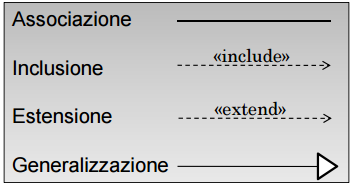
\includegraphics[width=0.75\columnwidth]{img9}

Inclusione ed estensione hanno degli aspetti in comune. L'inclusione è senza alcuna condizione mentre l'estensione è condizionale.

Individuzione UC:
\begin{itemize}
	\item Definizione contesto;
	\item Identificazione attori;
	\item Identificazione obbiettivi da raggiungere per ogni attore;
	\item Valutare e raffinare attori e UC
	\item Trovare le relazioni(Inclusione, Estensione, Generalizzazione).
\end{itemize}

\end{document}